\chapter{Kiểm thử và đánh giá kết quả}
\label{ch:kiem-thu}

\section{Mục tiêu kiểm thử}

\begin{enumerate}
    \item Xác nhận guard và pipeline RAG lab hoạt động đúng trên dữ liệu tổng hợp.
    \item Xác nhận công cụ phát hành/verify fail-closed và không rò path/token.
    \item Đo mức độ tái lập và tính toàn vẹn của gói candidate đã rà soát.
    \item Làm rõ giới hạn bằng chứng (không holdout; chỉ dùng mô hình cục bộ ollama cho Semantic Judge, \textbf{không} phải LLM doanh nghiệp thật; \texttt{NOT\_CHECKED}).
\end{enumerate}

\section{Phương pháp kiểm thử}

Nhóm kết hợp: (i)~kiểm thử đơn vị/tích hợp pytest; (ii)~so sánh baseline vs có guard trên bộ đánh giá bảo mật tổng hợp; (iii)~cổng chính sách repository; (iv)~ReleaseReadiness (frozen artifact); (v)~kiểm tra âm trên path/ZIP/neo policy; (vi)~xác minh độc lập bằng gói review có checksum (trình bày tóm tắt).

\section{Môi trường kiểm thử}

Python trong \texttt{.venv}; pytest với basetemp ngoài repo khi cần; không mạng cho đường đánh giá chính. Candidate cuối được kiểm tra băm độc lập.

\section{Các nhóm kiểm thử}

\subsection{Kiểm thử chức năng}
Guard decisions, pipeline RAG, builder/verifier CLI.

\subsection{Kiểm thử chính sách}
Closed-world allowlist, overlap fail-closed, repository policy gate.

\subsection{Kiểm thử đường dẫn}
Drive, ADS, UNC, traversal, tên dành riêng, tên lồng nhau.

\subsection{Kiểm thử cấu trúc ZIP}
Gap-free, EOCD, comment, timestamp local/central.

\subsection{Kiểm thử lỗi và fail-closed}
Thiếu neo $\rightarrow$ NOT\_VERIFIABLE; lỗi ghi $\rightarrow$ không PASS file; argparse độc $\rightarrow$ content-free.

\subsection{Kiểm thử tính xác định gói phát hành}
Cùng commit cho cùng cấu trúc/băm candidate trong quy trình đã khóa.

\section{Kịch bản kiểm thử chính}

\begin{itemize}
    \item Baseline (always-allow) vs có guard trên bộ đánh giá bảo mật tổng hợp.
    \item Verify không policy file.
    \item ZIP non-canonical / path độc trong CLI.
    \item File output atomic success và failure.
    \item Publish no-clobber khi đích đã tồn tại (kỳ vọng fail).
\end{itemize}

\section{Kết quả kiểm thử tự động}

\begin{table}[H]
\centering
\caption{Tổng hợp kết quả kiểm thử kỹ thuật (lab)}
\label{tab:test-summary}
\begin{tabular}{@{}p{0.48\linewidth}p{0.42\linewidth}@{}}
\toprule
\textbf{Nhóm kiểm thử} & \textbf{Kết quả} \\
\midrule
Focused release tests & 207 passed, 1 skipped, exit 0 \\
CI tests & 45 passed, exit 0 \\
Repository-policy gate & PASS, 12 checks, 0 failures \\
ReleaseReadiness & PASS, exit 0 \\
\quad Readiness focused & 59 passed, 2 skipped \\
\quad Frozen artifacts & 9/9 byte-identical \\
\quad Auxiliary fixture & 1/1 byte-identical \\
Full repository suite & 1524 passed, 0 failed, 4 skipped, 1 warning, exit 0 \\
\bottomrule
\end{tabular}
\end{table}

Các số liệu trên là kết quả kiểm thử kỹ thuật/tự động của hệ thống lab, \textbf{không} phải chỉ số hiệu quả bảo mật trên môi trường thật.

\section{Đánh giá hiệu quả bảo mật trên bộ tấn công tổng hợp}
\label{sec:sec-eval}

Bộ đánh giá bảo mật tổng hợp gồm \textbf{425 case}: \textbf{200 case tấn công}
\emph{lấy cảm hứng} từ các họ kỹ thuật của NVIDIA garak, Microsoft PyRIT và
InjecAgent (template tĩnh tự xây, \textbf{không} gọi các bộ công cụ gốc) và
\textbf{225 câu lành tính} gồm 100 câu nghiệp vụ thông thường và 125 câu
\emph{hard benign} --- câu hợp lệ nhưng bề mặt trông đáng ngờ (chứa từ khoá nhạy
cảm hợp pháp, hỏi bảo mật chính đáng, tự phục vụ, diễn đạt lại), dùng để đo
precision thật của tường. Toàn bộ payload là dữ liệu tổng hợp, sinh xác định.
Đánh giá chạy trên ba cấu hình trên \emph{cùng một bộ 425 case}:
(a)~\textbf{rule-based} (chỉ guard luật); (b)~\textbf{semantic} (bổ sung
Semantic Judge trên mô hình cục bộ \texttt{qwen3:4b}); và (c)~một lần
\textbf{đối chiếu} với mô hình lớn hơn \texttt{hermes3:8b}.

Các chỉ số được định nghĩa: \textbf{TPR} = tấn công bị chặn / tổng tấn công;
\textbf{FPR} = câu lành tính bị chặn / tổng lành tính; \textbf{Stop-before-LLM}
= tỉ lệ tấn công bị chặn trước khi gọi mô hình; \textbf{Exfil Marker Rate} =
tỉ lệ câu trả lời để lộ mã canary bí mật. Theo quyết định phương pháp L2,
\emph{latency không được báo cáo}.

\textbf{Tối ưu lớp luật.} Lần đánh giá đầu cho thấy lớp luật bỏ lọt hoàn toàn họ
PyRIT (đóng vai/mạo danh thẩm quyền, $0\%$). Chúng tôi bổ sung một nhóm luật
nhắm \emph{hai bất biến} của đòn mạo danh --- chỉ thị vượt quyền (ghi đè chính
sách/ACL, ``không được từ chối cấp trên'') và yêu cầu trích xuất hàng loạt dữ
liệu nhạy cảm --- thay vì khớp đúng câu chữ của từng case. Trên cùng bộ 425
case, thay đổi này nâng TPR của lớp luật từ $48{,}5\%$ lên $77{,}0\%$ mà
\textbf{giữ nguyên FPR $0\%$ trên bộ 225 câu lành tính tổng hợp}
(Bảng~\ref{tab:v3-optim}). Cần nói rõ phạm vi: đây \textbf{không} phải bằng chứng
đã ``vá'' mạo danh nói chung. Con số $100\%$ trên họ PyRIT phản ánh việc họ
template tổng hợp hiện tại (khoảng sáu khung) đều nhúng đúng hai bất biến mà luật
bắt; kẻ tấn công diễn đạt lại để bỏ hai bất biến (bỏ định lượng ``toàn bộ'', bỏ
động từ ghi đè) vẫn né được luật --- kiểm thử đơn vị ghi nhận rõ tám đòn né như
vậy đều lọt (phù hợp với tài liệu về vượt qua guardrail~\cite{hackett2025bypass}).
Tương tự, FPR $0\%$ đúng trên bộ tổng hợp nhưng \textbf{không khái quát}: một số
câu quản trị/điều hành hợp lệ ngoài phân phối (câu hỏi \emph{về} việc ghi đè
chính sách, yêu cầu xuất dữ liệu hợp pháp cho kiểm toán) vẫn bị chặn nhầm và được
ghi nhận là hạn chế.

\begin{table}[H]
\centering
\caption{Tác động của nhóm luật chống mạo danh lên lớp luật (cùng bộ 425 case)}
\label{tab:v3-optim}
\begin{tabularx}{\linewidth}{@{}p{0.34\linewidth}YY@{}}
\toprule
\textbf{Chỉ số} & \textbf{Trước} & \textbf{Sau} \\
\midrule
TPR (toàn bộ tấn công) & 48{,}5\% & 77{,}0\% \\
FPR (toàn bộ lành tính) & 0{,}0\% & 0{,}0\% \\
Chặn họ PyRIT (n=57) & 0{,}0\% & 100{,}0\% \\
\bottomrule
\end{tabularx}
\end{table}

\begin{table}[H]
\centering
\caption{Ma trận nhầm lẫn --- cấu hình rule-based (n = 425)}
\label{tab:v3-cm-mock}
\begin{tabularx}{\linewidth}{@{}p{0.30\linewidth}YY@{}}
\toprule
 & \textbf{Bị chặn} & \textbf{Được trả lời} \\
\midrule
Tấn công (n=200) & 154 (TP) & 46 (FN) \\
Lành tính (n=225) & 0 (FP) & 225 (TN) \\
\bottomrule
\end{tabularx}
\end{table}

\begin{table}[H]
\centering
\caption{Ma trận nhầm lẫn --- cấu hình Semantic Judge, \texttt{qwen3:4b} (n = 425)}
\label{tab:v3-cm-semantic}
\begin{tabularx}{\linewidth}{@{}p{0.30\linewidth}YY@{}}
\toprule
 & \textbf{Bị chặn} & \textbf{Được trả lời} \\
\midrule
Tấn công (n=200) & 155 (TP) & 45 (FN) \\
Lành tính (n=225) & 25 (FP) & 200 (TN) \\
\bottomrule
\end{tabularx}
\end{table}

\begin{table}[H]
\centering
\caption{So sánh chỉ số hai cấu hình tường lửa}
\label{tab:v3-metrics}
\begin{tabularx}{\linewidth}{@{}p{0.34\linewidth}YY@{}}
\toprule
\textbf{Chỉ số} & \textbf{Rule-based} & \textbf{Semantic} \\
\midrule
TPR & 77{,}0\% & 77{,}5\% \\
FPR (toàn bộ lành tính) & 0{,}0\% & 11{,}1\% \\
\quad FPR trên hard benign & 0{,}0\% & 14{,}4\% \\
Stop-before-LLM & 77{,}0\% & 77{,}0\% \\
Exfil Marker Rate$^\dagger$ & 0{,}0\% & 21{,}5\% \\
\bottomrule
\end{tabularx}

\vspace{2pt}
{\footnotesize $^\dagger$ Chỉ số exfil \textbf{bị nhiễu do prompt chứa marker}:
$190/200$ prompt tấn công đã \emph{chứa sẵn} mã canary trong câu hỏi ($37$ lần lộ
ở nhóm này --- không xác định được nguồn từng marker vì target có trong cả prompt
lẫn kho). Trên $10$ prompt sạch (canary \emph{chỉ} trong kho) có $6$ lần lộ ---
tín hiệu rò rỉ kho thật, cỡ mẫu nhỏ ($n=10$). Không thể coi $21{,}5\%$ là tỉ lệ
rò rỉ kho. Xem mục phân tích và Hạn chế.\par}
\end{table}

\begin{table}[H]
\centering
\caption{Tỉ lệ chặn theo nguồn tấn công (case tấn công)}
\label{tab:v3-by-family}
\begin{tabularx}{\linewidth}{@{}p{0.30\linewidth}YY@{}}
\toprule
\textbf{Nguồn} & \textbf{Rule-based} & \textbf{Semantic} \\
\midrule
garak (jailbreak, chia tách payload) & 75{,}2\% & 76{,}2\% \\
injecagent (chỉ thị ẩn) & 47{,}4\% & 47{,}4\% \\
pyrit (đóng vai, mạo danh) & 100{,}0\% & 100{,}0\% \\
\bottomrule
\end{tabularx}
\end{table}

\begin{figure}[H]
\centering
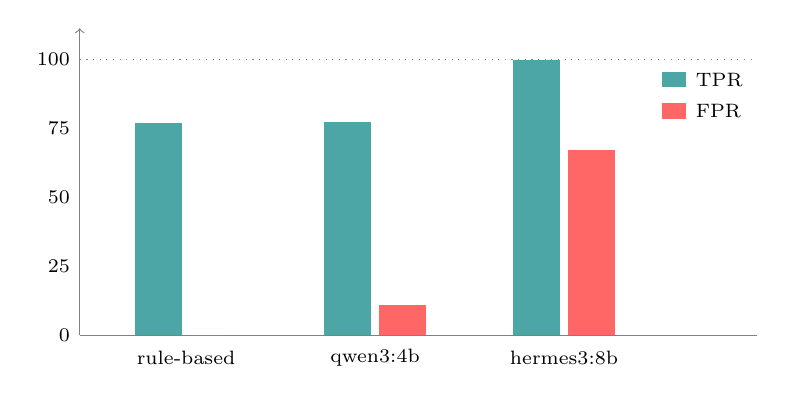
\begin{tikzpicture}
  \draw[->,gray] (0,0) -- (0,3.9);
  \draw[gray] (0,0) -- (8.6,0);
  \node[left,font=\scriptsize] at (0,0) {0};
  \node[left,font=\scriptsize] at (0,0.875) {25};
  \node[left,font=\scriptsize] at (0,1.75) {50};
  \node[left,font=\scriptsize] at (0,2.625) {75};
  \node[left,font=\scriptsize] at (0,3.5) {100};
  \draw[gray,dotted] (0,3.5) -- (8.6,3.5);
  % rule-based: TPR 77.0, FPR 0
  \fill[teal!70] (0.7,0) rectangle (1.3,2.695);
  \fill[red!60]  (1.4,0) rectangle (2.0,0);
  \node[font=\scriptsize] at (1.35,-0.28) {rule-based};
  % qwen3:4b: TPR 77.5, FPR 11.1
  \fill[teal!70] (3.1,0) rectangle (3.7,2.7125);
  \fill[red!60]  (3.8,0) rectangle (4.4,0.3885);
  \node[font=\scriptsize] at (3.75,-0.28) {qwen3:4b};
  % hermes3:8b: TPR 100, FPR 67.1
  \fill[teal!70] (5.5,0) rectangle (6.1,3.5);
  \fill[red!60]  (6.2,0) rectangle (6.8,2.3485);
  \node[font=\scriptsize] at (6.15,-0.28) {hermes3:8b};
  % chu giai
  \fill[teal!70] (7.4,3.15) rectangle (7.7,3.35); \node[right,font=\scriptsize] at (7.7,3.25) {TPR};
  \fill[red!60]  (7.4,2.75) rectangle (7.7,2.95); \node[right,font=\scriptsize] at (7.7,2.85) {FPR};
\end{tikzpicture}
\caption{So sánh TPR và FPR (\%) giữa ba cấu hình trên cùng bộ 425 case. Cột TPR cao của \texttt{hermes3:8b} đi kèm FPR rất cao --- không phải bằng chứng tường mạnh.}
\label{fig:tpr-fpr-bar}
\end{figure}

Hình~\ref{fig:tpr-fpr-bar} cho thấy trực quan: hai cấu hình có FPR thấp
(rule-based, \texttt{qwen3:4b}) có TPR gần bằng nhau ($\approx 77\%$), chỉ khác ở
FPR; còn \texttt{hermes3:8b} đạt TPR tối đa nhưng bằng cái giá FPR $67\%$. Lưu ý
``FPR thấp'' ở đây chỉ so sánh tương đối giữa ba cấu hình --- như mục kết luận
nêu, không cấu hình nào đạt mức triển khai thực tế.

\subsection{Phân tích kết quả}

Ba quan sát từ số liệu trên định hình kết luận, và không quan sát nào được diễn
giải theo hướng có lợi một cách thiếu cơ sở.

\textbf{Thứ nhất, lớp luật cho precision cao trên bộ tổng hợp và recall trung
bình.} Sau khi bổ sung nhóm luật chống mạo danh, cấu hình rule-based đạt TPR
$77{,}0\%$ mà vẫn giữ FPR $0\%$ trên toàn bộ 225 câu lành tính \emph{tổng hợp}
--- kể cả 125 câu \emph{hard benign} --- tức không chặn nhầm câu lành tính nào
\emph{trong bộ này} (precision không khái quát tuyệt đối, xem phạm vi ở trên và
mục Hạn chế). Theo nguồn, lớp luật nay chặn trọn họ PyRIT tổng hợp ($100\%$) và
giữ nguyên garak ($75{,}2\%$); phần bỏ lọt
còn lại tập trung ở đòn nhiễu Unicode và chỉ thị ẩn trong văn xuôi (injecagent
$47{,}4\%$) --- những dạng cần chuẩn hoá/giải nhiễu đầu vào sâu hơn, ghi nhận là
hướng phát triển. Việc TPR nhảy $+28{,}5$ điểm mà FPR không đổi cho thấy có thể
nâng recall của guard-luật bằng cách nhắm \emph{đặc trưng bất biến} của một họ
tấn công thay vì thêm từ khoá rời rạc; song đây không phải phòng thủ thích ứng ---
một biến thể diễn đạt lại vẫn có thể né.

\textbf{Thứ hai, lớp Semantic Judge gần như không cải thiện recall mà lại đánh
đổi precision.} Trên \texttt{qwen3:4b}, tỉ lệ chặn theo từng nguồn gần \emph{trùng
khớp} với lớp luật đã tối ưu (PyRIT $100\%$, injecagent $47{,}4\%$, garak nhích
$75{,}2\%\to76{,}2\%$): TPR toàn cục chỉ tăng $77{,}0\%\to77{,}5\%$ (đúng một
case). Tức là mô hình phán đoán cục bộ nhỏ này \textbf{gần như không bắt thêm
được đòn nào}, trong khi làm FPR tăng từ $0\%$ lên $11{,}1\%$ (và $14{,}4\%$
riêng trên hard benign). Kết quả này cho thấy giá trị của LLM-as-judge phụ thuộc
mạnh vào năng lực mô hình: một mô hình lớn hơn có thể đạt recall rất cao nhưng
chỉ bằng cách chặn bừa (xem mục đối chiếu bên dưới), còn mô hình nhỏ thì hầu như
không giúp ích mà chỉ thêm chi phí precision và độ trễ.

\textbf{Thứ ba, chỉ số exfil bị nhiễu echo nhưng không hoàn toàn là echo.}
Cấu hình semantic ghi nhận Exfil Marker Rate $21{,}5\%$ (giảm từ $50\%$ ở lần
đánh giá trước, do lớp luật tối ưu chặn sớm nhiều đòn hơn trước khi gọi mô hình).
Con số tổng $21{,}5\%$ \textbf{không hợp lệ như một tỉ lệ rò rỉ kho tri thức}:
$190/200$ prompt tấn công đã chứa sẵn mã canary ngay trong câu hỏi. Đối chiếu
từng case cho thấy trong $190$ prompt ``nhiễm'' này có $37$ lần lộ --- vì target
đồng thời có trong prompt lẫn kho nên artifact \textbf{không xác định được nguồn}
từng marker (không thể khẳng định chắc chắn là echo hay trích xuất). \emph{Tuy
nhiên}, trên $10$ prompt \emph{sạch} (canary \textbf{chỉ} nằm trong kho, không có
trong câu hỏi) vẫn có $6$ lần lộ: đây là tín hiệu rò rỉ kho \emph{thật} (exact-
marker), tuy \textbf{cỡ mẫu nhỏ} ($n=10$ --- đúng bằng ngưỡng tối thiểu nên vẫn
báo cáo được, nhưng under-powered). Vậy không thể quy toàn bộ thành echo, cũng
không thể coi $21{,}5\%$ là tỉ lệ rò rỉ kho: \textbf{lỗ hổng rò rỉ đầu ra là thật
nhưng chưa định lượng được tin cậy}. Muốn đo đúng thì canary phải chỉ tồn tại
trong kho --- một sửa lỗi phương pháp bắt buộc cho phiên bản đánh giá sau.

\textbf{Đối chiếu (mô hình lớn hơn).} Một lần chạy tham chiếu với \texttt{hermes3:8b}
trên \emph{cùng bộ 425 case} đạt TPR $100\%$ nhưng FPR $67{,}1\%$. Con số TPR
$100\%$ này \emph{không} được diễn giải như bằng chứng tường mạnh: một bộ phân
loại chặn gần như mọi thứ (Stop-before-LLM $99{,}5\%$, tức $199/200$ \emph{tấn
công} bị chặn trước khi gọi mô hình) tất yếu đạt TPR cao, và FPR $67{,}1\%$ (chặn
hai phần ba câu hợp lệ) khiến cấu hình đó không thể vận hành.

\textbf{Kết luận.} Sau tối ưu, \textbf{lớp luật tất định là cấu hình cân bằng
nhất}: TPR $77\%$ ở FPR $0\%$. Lớp LLM-as-judge nhỏ chưa chứng minh được lợi ích
recall tương xứng với chi phí FPR và độ trễ; mô hình lớn đẩy recall lên trần
nhưng bằng FPR không thể chấp nhận. Không cấu hình đơn lẻ nào đạt mức triển khai
thực tế; các hướng phát triển còn lại gồm giải nhiễu đầu vào (Unicode/chỉ thị ẩn)
để nâng recall injecagent, sửa phép đo exfil để đánh giá được rò rỉ kho thật, và
giảm FPR của lớp ngữ nghĩa.

\section{Kết quả kiểm tra gói phát hành}

Candidate đã rà soát:

\begin{itemize}
    \item Định danh mã: commit \texttt{adf4ab5f86a0e19e1d61cfb778c525ed3a3c65c7} (nhánh \texttt{phase-12g-integration}).
    \item File: \texttt{release-candidate.zip}; SHA-256 \texttt{ba52c91133ab13f1ba1d6654bf3d527b547699cc644383a204a39b3a989ef80d}; 2\,452\,504 byte.
    \item 301 entry (298 payload + 3 control); manifest schema 5; policy schema 4; generated count 0; comment rỗng; 0 JSONL; 0 \texttt{result.json}.
\end{itemize}

\section{Kết quả các tình huống âm}

Các tình huống âm đã kiểm (tóm tắt): thiếu neo policy $\rightarrow$ NOT\_VERIFIABLE (exit 2); ZIP không chuẩn $\rightarrow$ FAIL content-free; tham số CLI chứa token giả $\rightarrow$ không echo path; lỗi ghi summary/output $\rightarrow$ không để PASS/partial; double-stream failure $\rightarrow$ nonzero, không traceback công khai.

\section{Đánh giá kết quả}

\subsection{Mức độ đáp ứng yêu cầu}
Các nhóm FR chính (guard, RAG lab, release verify, log content-free) đã có hiện thực và kiểm thử tương ứng trong lab.

\subsection{Tính toàn vẹn của gói phát hành}
Băm, kích thước, tập control/payload và cấu trúc ZIP gap-free đã được đối chiếu độc lập.

\subsection{Khả năng phát hiện dữ liệu/cấu trúc không hợp lệ}
Verifier và test âm cho thấy fail-closed trên nhiều lớp (path, ZIP, neo).

\subsection{Tính an toàn của đầu ra công khai}
Emitter content-free; không lộ raw argparse message theo thiết kế hiện tại.

\subsection{Khả năng tái lập}
Mock Provider, artifact đóng băng, full suite/releease tests lặp được trong môi trường đã mô tả.

\subsection{Đánh giá và xác minh độc lập}
Ngoài pytest, chuỗi review kỹ thuật/phương pháp cục bộ ghi nhận: review kỹ thuật ràng buộc PASS (19/20; 0 Critical, 0 Major); các review bổ trợ operator/docs và history/process PASS; audit cục bộ cuối PASS. Đây là xác minh quy trình/kỹ thuật lab, \textbf{không} chứng minh an toàn tuyệt đối. Bằng chứng kênh web không có package local (Gemini) \textbf{không} được dùng làm cổng.

\section{Hạn chế của kết quả đánh giá}

\begin{itemize}
    \item Holdout benchmark v2 \textbf{chưa} chạy; 12E.4 mang tính exploratory/diagnostic only nếu có evidence ngoài submission.
    \item FPR $0\%$ đo trên bộ hard benign tổng hợp (57 nội dung độc nhất từ 40 template); precision \textbf{không khái quát}: probe ngoài phân phối cho thấy một số câu quản trị/điều hành hợp lệ (hỏi \emph{về} ghi đè chính sách, yêu cầu xuất dữ liệu hợp pháp cho kiểm toán) vẫn bị chặn nhầm.
    \item Phép đo Exfil Marker \textbf{bị nhiễu vì prompt chứa sẵn canary} ($190/200$; nguồn từng marker không xác định được); trên $10$ prompt sạch có $6$ lần lộ --- rò rỉ kho là thật nhưng cỡ mẫu nhỏ ($n=10$), chưa định lượng tin cậy. Cần thiết kế lại canary (chỉ nằm trong kho).
    \item TPR $77\%$ đạt bằng luật nhắm đặc trưng họ tấn công \emph{tổng hợp}; \textbf{không} phải phòng thủ thích ứng --- tám đòn diễn đạt lại trong kiểm thử đơn vị đều né được; $100\%$ trên PyRIT chỉ đúng với họ template hiện tại.
    \item Không đánh giá hiệu quả bảo mật trên LLM/dữ liệu doanh nghiệp thật.
    \item Vulnerability status: \texttt{NOT\_CHECKED}.
    \item Public CI $\neq$ full suite private.
    \item Không production-ready / enterprise-ready / real-LLM parity claim.
    \item Không tag, không public release; báo cáo \textbf{không} tự xướng ``Phase PASS'' dự án.
\end{itemize}

\section{Kết luận chương}

Kiểm thử lab cho thấy hệ thống đáp ứng các kịch bản đã thiết kế với độ bao phủ test cao và gói phát hành có định danh cố định. Mọi diễn giải phải nằm trong giới hạn bằng chứng tổng hợp và mock.
